\section{Задание 1. Аппроксимация двумерной гауссианой}

\subsection{Постановка задачи}

Дана таблица экспериментальных данных (Вариант 7):

\begin{table}[H]
    \centering
    \caption{Исходные данные}
    \label{tab:data}
    \begin{tabular}{|c|c|c|c|}
        \hline
        \textbf{Точка} & \textbf{$x$} & \textbf{$y$} & \textbf{$z$} \\
        \hline
        0 & 1.10 & 1.10 & 0.29 \\
        1 & 2.01 & 1.98 & 1.24 \\
        2 & 3.01 & 2.85 & 4.94 \\
        3 & 3.86 & 3.99 & 4.72 \\
        4 & 5.10 & 4.90 & 0.77 \\
        \hline
    \end{tabular}
\end{table}

Требуется аппроксимировать зависимость $z = f(x, y)$ двумерной функцией Гаусса.

\subsection{Заполнение пропусков в программном модуле}

В предоставленном шаблоне на языке Python необходимо заполнить следующие пропуски:

\begin{enumerate}
    \item \textbf{Извлечение признаков:}
    \begin{verbatim}
    X = data[:, 0]
    Y = data[:, 1]
    Z = data[:, 2]
    \end{verbatim}

    \item \textbf{Функция Гаусса (ветвь без поворота):}
    \begin{verbatim}
    x_new = x - x0
    y_new = y - y0
    exp_part = np.exp(-((x_new**2)/(2*sigma_x**2)
                        + (y_new**2)/(2*sigma_y**2)))
    \end{verbatim}

    \item \textbf{Функция потерь:}
    \begin{verbatim}
    A, x0, y0, sigma_x, sigma_y, theta, offset = model_params
    pred = gauss_2d(X[i], Y[i], A, x0, y0,
                     sigma_x, sigma_y, theta, offset)
    errors = (np.array(predictions) - Z) ** 2
    mse = 0.5 * np.mean(errors)
    \end{verbatim}

    \item \textbf{Начальное приближение:}
    \begin{verbatim}
    max_idx = np.argmax(Z)
    A_start = Z[max_idx] + 0.1
    x0_start = X[max_idx]
    y0_start = Y[max_idx]
    \end{verbatim}

    \item \textbf{Верификация:}
    \begin{verbatim}
    pred = gauss_2d(X[i], Y[i], A_opt, x0_opt, y0_opt,
                     sigma_x_opt, sigma_y_opt, theta_opt, offset_opt)
    \end{verbatim}

    \item \textbf{Визуализация:}
    \begin{verbatim}
    Z_grid[i, j] = gauss_2d(X_grid[i, j], Y_grid[i, j],
         A_opt, x0_opt, y0_opt, sigma_x_opt, sigma_y_opt,
         theta_opt, offset_opt)
    \end{verbatim}
\end{enumerate}

\subsection{Математическая модель}

Двумерная функция Гаусса с поворотом:

\begin{equation}\label{eq:gauss}
    z(x, y) = A \cdot \exp\left(-Q\right) + b,
\end{equation}
\begin{equation}
    Q = \frac{x_{new}^2}{2\sigma_x^2} + \frac{y_{new}^2}{2\sigma_y^2},
\end{equation}
\begin{equation}
    \begin{cases}
        x_{new} = (x - x_0)\cos\theta + (y - y_0)\sin\theta \\
        y_{new} = -(x - x_0)\sin\theta + (y - y_0)\cos\theta
    \end{cases}
\end{equation}

Вектор параметров: $\mathbf{p} = (A, x_0, y_0, \sigma_x, \sigma_y, \theta, b)$.

\subsection{Метод оптимизации}

Минимизация функции потерь MSE:
\begin{equation}
    L(\mathbf{p}) = \frac{1}{2N}\sum_{i=1}^{N}\left(z(x_i, y_i; \mathbf{p}) - z_i\right)^2 \to \min_{\mathbf{p}}
\end{equation}

Метод: \textbf{L-BFGS-B} (квазиньютоновский метод с ограниченной памятью и границами).

Начальное приближение: $A_0 = z_{\max} + 0.1 = 5.04$, центр --- в точке максимума $(3.01, 2.85)$, $\sigma_{x,0} = \sigma_{y,0} = 0.5 \cdot \text{std}$, $\theta_0 = 0$, $b_0 = 0$.

\subsection{Результаты}

\begin{table}[H]
    \centering
    \caption{Оптимальные параметры гауссовой модели}
    \label{tab:gauss_params}
    \begin{tabular}{|c|c|}
        \hline
        \textbf{Параметр} & \textbf{Значение} \\
        \hline
        $A$ & 5.5516 \\
        $x_0$ & 3.4413 \\
        $y_0$ & 3.3033 \\
        $\sigma_x$ & 0.9118 \\
        $\sigma_y$ & 1.7552 \\
        $\theta$ & 0.1180 рад (6.76°) \\
        $b$ & 0.2348 \\
        \hline
        Число итераций & 26 \\
        \hline
    \end{tabular}
\end{table}

\subsection{Аналитический вид модели}

\begin{equation}\label{eq:gauss_result}
    z(x, y) = 5.5516 \cdot \exp\left(-\frac{(x - 3.4413)^2}{2 \cdot 0.9118^2} - \frac{(y - 3.3033)^2}{2 \cdot 1.7552^2}\right) + 0.2348,
\end{equation}
с предварительным поворотом координат на угол $\theta = 6.76^\circ$.

\subsection{Таблица невязок}

\begin{table}[H]
    \centering
    \caption{Невязки гауссовой модели}
    \label{tab:gauss_residuals}
    \begin{tabular}{|c|c|c|c|c|c|}
        \hline
        \textbf{Точка} & \textbf{$x$} & \textbf{$y$} & \textbf{$z_{факт}$} & \textbf{$z_{модель}$} & \textbf{Невязка} &  \textbf{Кв. невязки} \\
        \hline
        0 & 1.10 & 1.10 & 0.29 & 0.2900 & $4.0 \times 10^{-6}$ & $1.6 \times 10^{-11}$ \\
        1 & 2.01 & 1.98 & 1.24 & 1.2400 & $-1.9 \times 10^{-5}$ & $3.6 \times 10^{-10}$ \\
        2 & 3.01 & 2.85 & 4.94 & 4.9400 & $-1.1 \times 10^{-5}$ & $1.2 \times 10^{-10}$ \\
        3 & 3.86 & 3.99 & 4.72 & 4.7200 & $4.0 \times 10^{-6}$ & $1.6 \times 10^{-11}$ \\
        4 & 5.10 & 4.90 & 0.77 & 0.7700 & $2.5 \times 10^{-5}$ & $6.3 \times 10^{-10}$ \\
        \hline
    \end{tabular}
\end{table}

MSE $= 2.3 \times 10^{-10}$, RMSE $= 1.5 \times 10^{-5}$. Все невязки пренебре-жимо малы, что указывает на точное совпадение модели с данными.

\subsection{Визуализация}

\begin{figure}[H]
    \centering
    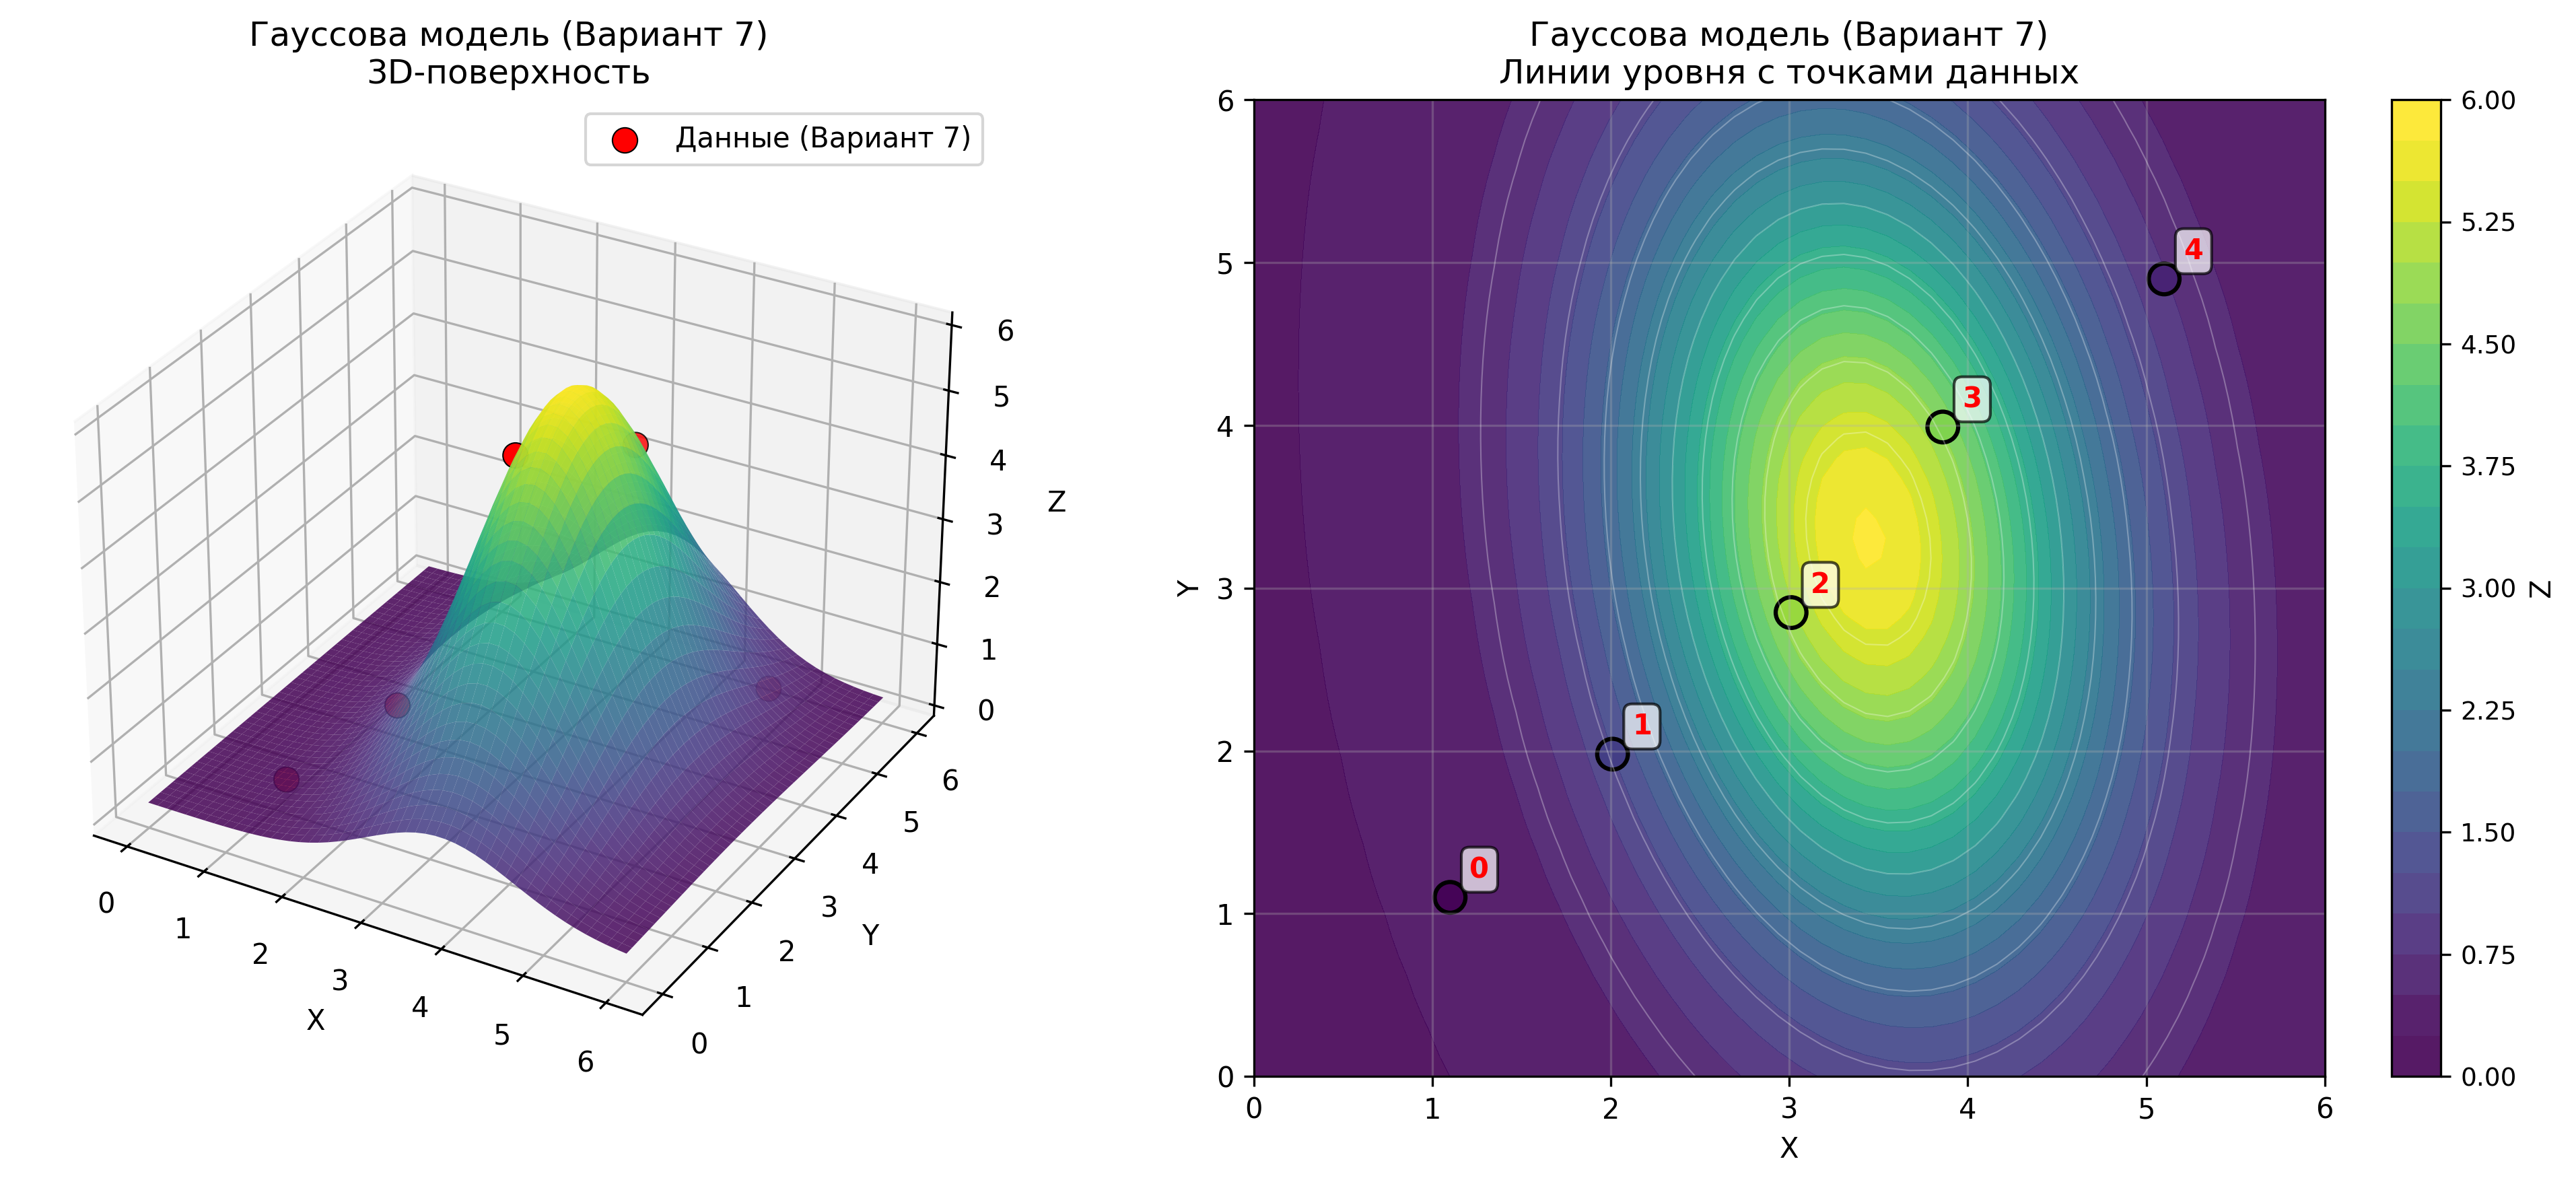
\includegraphics[width=\textwidth]{pic/gaussian_model.png}
    \caption{Гауссова модель: 3D-поверхность (слева) и линии уровня с точками данных (справа)}
    \label{fig:gauss_model}
\end{figure}

Модельная поверхность имеет колоколообразную форму. Экспериментальные точки (красные) лежат непосредственно на поверхности, линии уровня проходят через соответствующие точки. Небольшой поворот ($\theta = 6.76^\circ$) отражает асимметрию данных.

\subsection{Вывод}

Гауссова модель с 7 параметрами обеспечивает практически точную аппроксимацию данных варианта 7. Полученные невязки имеют порядок $10^{-5}$ и менее, что подтверждает гауссову природу исходных данных.
